\chapter{Exercise 08}
%******************************************************************************%
%                                                                              %
%                                 Interlude                                    %
%                         for Machine Learning module                          %
%                                                                              %
%******************************************************************************%

\section*{Interlude - Fifty Shades of Linear Algebra}

In the last exercise, we implemented the loss function in two subfunctions.
It worked, but it's not very pretty.
What if we could do it all in one step, with linear algebra?   

As we did with the hypothesis, we can use a vectorized equation to improve the calculations of the loss function.

So now let's look at how squaring and averaging can be performed (more or less) in a single matrix multiplication!

$$
J(\theta) = \frac{1}{2m}\sum_{i=1}^{m}(\hat{y}^{(i)} - y^{(i)})^2
$$
$$
J(\theta) = \frac{1}{2m}\sum_{i=1}^{m}[(\hat{y}^{(i)} - y^{(i)}) (\hat{y}^{(i)} - y^{(i)})]
$$

Now, if we apply the definition of the dot product:

$$
J(\theta) = \frac{1}{2m}(\hat{y} - y) \cdot(\hat{y}- y)
$$
\newpage
\extitle{Lets Make Nice Plots Again}
\turnindir{ex08}
\exnumber{08}
\exfiles{plot.py}
\exforbidden{None}
\makeheaderfilesforbidden


% ================================= %
\section*{Objective}
% --------------------------------- %
You must implement a function which plots the data, the prediction line, and the loss.  
You will plot the $x$ and $y$ coordinates of all data points as well as the prediction line generated by your theta parameters.
Your function must also display the overall loss ($J$) in the title, and draw small lines marking the distance between each data point and its predicted value.

% ================================= %
\section*{Instructions}
% --------------------------------- %
In the plot.py file create the following function as per the instructions given below:
\begin{minted}[bgcolor=darcula-back,formatcom=\color{lightgrey},fontsize=\scriptsize]{python}
def plot_with_loss(x, y, theta):
"""Plot the data and prediction line from three non-empty numpy.ndarray.
    Args:
      x: has to be an numpy.ndarray, one-dimensional array of size m.
      y: has to be an numpy.ndarray, one-dimensional array of size m.
      theta: has to be an numpy.ndarray, one-dimensional array of size 2.
    Returns:
        Nothing.
    Raises:
      This function should not raise any Exception.
    """
    ... Your code ...
\end{minted}

\newpage

% ================================= %
\section*{Examples}
% --------------------------------- %
\begin{minted}[bgcolor=darcula-back,formatcom=\color{lightgrey},fontsize=\scriptsize]{python}
import numpy as np
x = np.arange(1,6)
y = np.array([11.52434424, 10.62589482, 13.14755699, 18.60682298, 14.14329568])

# Example 1:
theta1= np.array([18,-1])
plot_with_loss(x, y, theta1)
# Output:
\end{minted}

\begin{figure}[H]
  \centering
  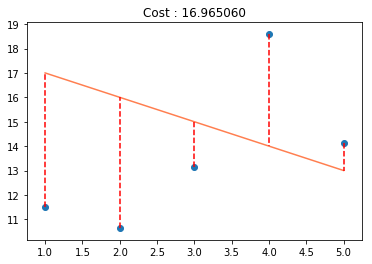
\includegraphics[scale=0.65]{assets/plotcost1.png}
  \caption{Example 1}
\end{figure}

\begin{minted}[bgcolor=darcula-back,formatcom=\color{lightgrey},fontsize=\scriptsize]{python}
# Example 2:
theta2 = np.array([14, 0])
plot_with_loss(x, y, theta2)
# Output:
\end{minted}

\begin{figure}[H]
  \centering
  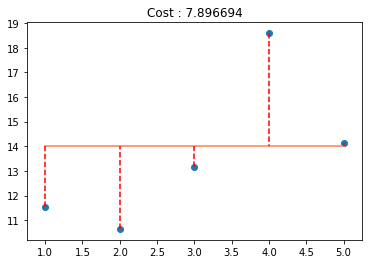
\includegraphics[scale=0.65]{assets/plotcost2.png}
  \caption{Example 2}
\end{figure}

\newpage

\begin{minted}[bgcolor=darcula-back,formatcom=\color{lightgrey},fontsize=\scriptsize]{python}
# Example 3:
theta3 = np.array([12, 0.8])
plot_with_loss(x, y, theta3)
# Output:
\end{minted}

\begin{figure}[H]
  \centering
  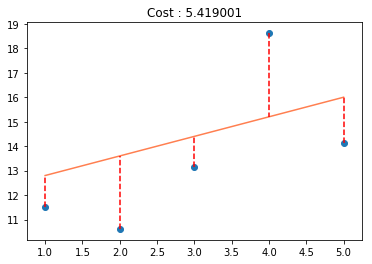
\includegraphics[scale=0.65]{assets/plotcost3.png}
  \caption{Example 3}
\end{figure}